\documentclass[border=4pt]{standalone}

\usepackage{tikz}

\definecolor{otblue}{HTML}{0072B2}
\definecolor{otorange}{HTML}{E69F00}
\definecolor{otteal}{HTML}{009E73}
\definecolor{otpurple}{HTML}{CC79A7}
\definecolor{otgray}{HTML}{5A5A5A}

\begin{document}
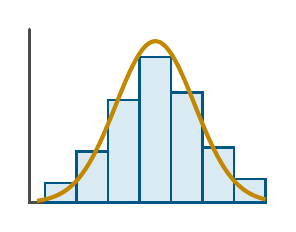
\begin{tikzpicture}[line width=0.9pt]
\draw[otgray!85!black, line width=1.2pt, line cap=round] (0,2.2) -- (0,0) -- (3,0);
  \foreach \x/\h in {0.2/0.25,0.6/0.65,1/1.3,1.4/1.85,1.8/1.4,2.2/0.7,2.6/0.3}{\filldraw[draw=otblue!75!black, fill=otblue!15] (\x,0) rectangle +(0.4,\h);}
  \draw[otorange!85!black, line width=1.5pt] plot[smooth, domain=0.1:3, samples=40] (\x,{2.05*exp(-((\x-1.6)^2)/0.5)});
\end{tikzpicture}
\end{document}
